% !TEX TS-program = pdflatexmk
%% This is an example first chapter.  You should put chapter/appendix that you
%% write into a separate file, and add a line \include{yourfilename} to
%% main.tex, where `yourfilename.tex' is the name of the chapter/appendix file.
%% You can process specific files by typing their names in at the 
%% \files=
%% prompt when you run the file main.tex through LaTeX.
\chapter{Introduction}

\section{The Standard Model}
The Standard Model (SM) was built in the late 70th of 20th century to  describe the matter compositions and interactions using a group of fundamental particles - fermions and bosons. 
In the Standard Model, there are three generations of quarks and leptons, along with their anti-particles, which are all fermions. On the other hand, the bosons in the Standard Model consist of gluons, photons, $W^{\pm}$ and $Z^0$ bosons that are all gauge bosons and one Higgs boson that is a scalar boson. This group of particles are summarized in Figure \ref{fig:sm-table}. The Standard Model depicts the interactions between elementary particles as the exchange of the bosons. The strong interaction requires the exchange of gluons. Photons, $W^{\pm}$ and $Z^0$ bosons carry the electromagnetic force and weak force, which are unified as electroweak interaction in the Standard Model. Higgs boson is responsible for the generation of masses for the gauge bosons through electroweak symmetry breaking\cite{aad2012observation}. The Standard Model has been proved to be an excellent theoretical model that can be used to explain many experimental observations, but sadly not all of them. For instance, neutrino mass is expected to be zero in the Standard Model but the flavor oscillation indicates non-zero mass of neutrinos. The observation of Charge-Parity ($\it{CP}$) asymmetry in universe presented by the absence of antimatter can not be fully explained by the $\it{CP}$ violation sources within the Standard Model. These experimental observations require further researches beyond the Standard Model, which is called New Physics (NP) studies. 
\begin{figure}[H]
	\centering
	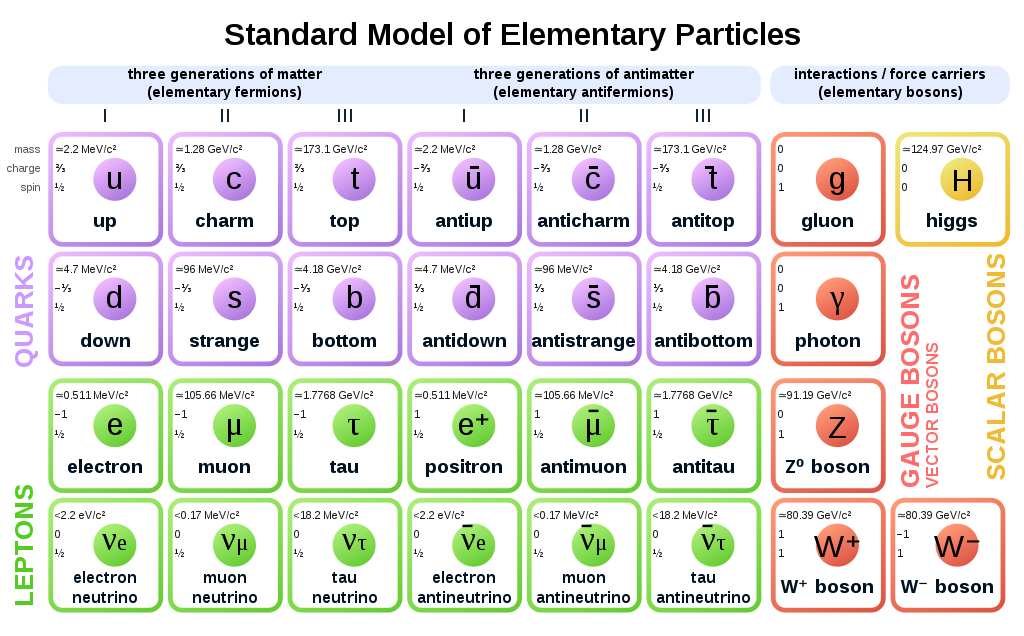
\includegraphics[height=9cm]{1024px-Standard_Model_of_Elementary_Particles_Anti.png}
	\caption{Elementary particles in the Standard Model.\cite{sm_particles}}
	\label{fig:sm-table}
\end{figure}

\begin{comment}
 in a picture where they interact through exchange of certain force carriers which are bosons as well. More specifically, each set of these carriers mediate one type of fundamental interaction. The force in which most of classical objects interact is electromagnetic interaction and it's mediated by photons. The force that plays a role in the $\beta$ decay is weak interaction, of which the mediators are $\textit{W}$ and $\textit{Z}$ bosons. When a proton and a neutron interact within a nuclei transforming into each other, the actual force carriers are 8 types of gluons (or $\pi$ mesons between nucleus), and it's called strong force. Last but not least, in the quantum field theory, all of these particles has zero mass if there's no spontaneous symmetry breaking by introducing one another boson - Higgs boson, in the Lagrangian formalism of all interactions. With this being said, the ``mass'' is taken as the weight of how strong all these particles interact with Higgs field.
 
 However, the S prediction does not perfectly match with experimental observations. Since the day theory was built, generations of particle physics experiments have been searching for evidences beyond the SM, as known as New Physics (NP). New Physics is expected to unfold a more profound truth of nature which hopefully explains these observed mismatches. The studies on these fields naturally draw a large attention from modern physicists, focusing on discovering and explaining the mismatches between the SM predictions and experiments. Among these research fields, the studies of symmetry violations (or called as asymmetries) plays an important role. The studies of symmetries was once the driving force for physicists when building the modern theory about particle physics. It is no wonder that now the violation of symmetries, which  physicists didn't expect to happen , has become the cutting edge research topics for New Physics. 
 
\end{comment}





\section{Symmetry Violation}
Symmetry violation has been one of the focuses in NP studies due to the internal link between symmetries and conservation laws, which makes it a good probe for possible NP theories beyond the SM. When a known symmetry is found to be broken, it usually leads to the discovery of a new theory.


There are three types of discrete symmetric operations which play important roles in particle physics. Charge-conjugation $\textit{C}$ is the operation that turns particle to its anti-particle. Parity transformation $\textit{P}$  is the one that puts a negative sign before all the spatial related vector such as $\overrightarrow{r} \to -\overrightarrow{r}$. The time-reversing operation $\textit{T}$ is to reversely proceed a physical process backward time.  Physicists were convinced that each of these three symmetric operations makes no change to any physics system. However, in 1950s, Lee and Yang \cite{PhysRev.104.254} first questioned that parity symmetry might be broken in weak interactions. They offered a few possible ways to test it and then by Wu \cite{Wu_exp}, an observation on the $\beta$ decay of $^{60}$Co was presented that the electrons emitted from  $^{60}$Co decay prefers the direction of nuclear spin that can be controlled by the external magnetic field. The violation of $P$ symmetry was discovered by this clear evidence. 

\begin{comment}
\begin{figure}[htbp]
\centering
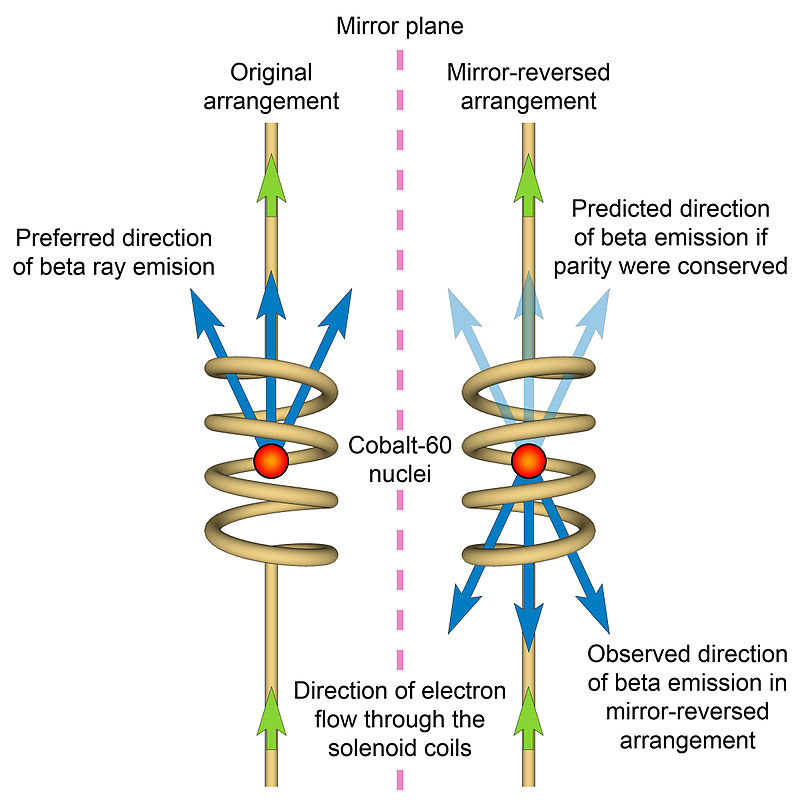
\includegraphics[height=8cm]{DsBxU.jpg}
\caption{$^{60}$Co decay violates the parity because of the unbalance of electron emissions\cite{wu_exp}}
\label{fig:Co60}
\end{figure}
\end{comment}

The first evidence of $CP$ violation was discovered in neutral $K^0$ system by Cronin and Fitch's experiment\cite{christenson1964evidence}. The neutral $K^0$ mesons can be observed as two states that have significantly different lifetime (called as ``$K_S^0$" and ``$K_L^0$" for short and long lifetime particles) with opposite $\it{CP}$ eigenvalue. The experiment measured the decay products at 57 foot of a neutral $K^0$ beamline assuming all the particle at the end of the beam should be long lifetime $K_L^0$, nearly no $K_S^0$. But 0.002\% of $K^0_L$ were found to decay into $\pi^+\pi^-$ which is the main decay process of $K_S^0$.($CP$ eigenvalue $=1$ in $\pi^+\pi^-$ final states, while $K_L$ has  $CP$ eigenvalue $=-1$ ). Given that the expected distance to have 0.002\% of $K_S^0$ at about speed of light is no more than 1 meter in the beamline, such a deviation at 57 foot is an obvious evidence that $K_L^0 \to \pi^+\pi^- $ exists and therefore $CP$ symmetry is violated in the neutral $K^0$ system.

In 1973, Kobayashi and Maskawa introduced a quark mixing matrix called CKM matrix for three or more generations of quarks before the discovery of the third generation of the quark family\cite{CKM}. The theory naturally explained an irreducible complex phase in CKM matrix and it accounts for the origin of $CP$ asymmetries of weak interactions in the Standard Model. The experimental evidence of $CP$ violation in $B$ meson system was observed in 2001 by Belle and BaBar experiments\cite{teramoto2002cp}\cite{langestudy}. They measured the time-dependent decay time difference of $B$ and $\bar{B}$ in the decay of $B\to J/\psi K_S^0$. This channel provided a good clearness in theoretical prediction and has relatively large branching fraction, thus it's called the ``golden mode"\cite{bigi1989question}. In 2008, Kobayashi and Maskawa were rewarded the Nobel Prize to highly value their contribution to $CP$ violation mechanism in the SM, to which Belle experiment contributes greatly. Later in 2010, the upgrade of Belle, Belle II and the upgrade of KEK accelerator, SuperKEKB, were approved to further push the understanding of $CP$ violation along with other topics in New Phsyics researches. 

\section{CKM mechanism}
\begin{comment}
Three kinds of fundamental interaction: weak, strong and electromagnetic interactions have been included in the SM. The SM can inherently solve the origin of the symmetries and asymmetries, with the theoretical support from quantum field theory (QFT). In QFT, the particles are treated as the excitation of its field and the interaction between particles can also be treated as the exchange of energy and momentum between particles. Enlighten by many aspects in classical mechanism, QFT is also built on a formalism in which the Lagrangian plays an essential role. The difference is field, as a physical entity, is universally distributed in space-time, whereas classical objects can only exist with a local position. Given this fact, it is natural to define the Lagrangian of field as a ``density" of Lagrangian of particles. In the SM, for instance, a fermion field $\it{\Psi}$ with mass $m$ is described by a field as follows:

\begin{equation}
\mathcal{L}_0 = \it{\overline{\Psi}(i\gamma^\mu \partial_\mu-m)\Psi}
\end{equation}

Such form presents a field which will fit in Lorentz transition and space-time transition. Then gauge theory is used to describe the interaction of fermions so that the Lagrangian should be invariant under the local gauge transformation. There are different types of local gauge transformations, as well as their invariance. 
Group is the mathematical term used to describe transformation invariance. Each group has a basic presentation of matrix. If every elements in a group can find a corresponding matrix which keeps their relations in multiplying operation,then the smallest dimension of such matrix is called basic matrix presentation. If the matrix elements are Unitary, n dimension, such group is called$\it{U}$(n), 
specially if the anti-matrix is the conjugation-transverse of itself, such group is called Special Unitary.($\it{SU}$(n)) 


For instance, in the U(1) gauge transition, if one requires the invariance of electromagnetism by adding $\it{U}$(1) gauge, the Maxwell formalism naturally fits in the quantum electroweak dynamics (QED), along with the weak interaction which is invariant under not only $\it{U}$(1) transformation but also $\it{SU}$(2). The symmetry of electromagnetic force and weak force is spontaneously broken due to the non-zero expected value of Higgs field of the vacuum. That makes the coupling of different field varied so the carriers of electromagnetic field and weak field diverged. Massless particle $\gamma$ is carrying the electromagnetic force. $W^{+/-}$ and neutral $Z$ deliver the force of weak interaction. They have different coupling strength to the Higgs field, which excites a neutral particle, Higgs boson $H$. The quarks, however, not only coupling to $W^{+/-},Z$ by weak interaction, they directly interact with each other by exchanging gluons by strong force. The strong interaction is described by $SU$(3) with eight types of different gluons, and every gluon has 3 colors. The mechanism that describes this interaction is called ``quantum chromodynamics" (QCD). 

The contribution of the origin of $CP$ violation is mainly from the weak current in the SM Lagrangian. So the discussion of the theoretical interface of $CP$ violation will be focusing on the weak interaction. In the Lagrangian formalism in the SM, gauge interactions are described by the terms in the Lagrangian in a form that quark field is coupling with each other through gauge current, specifically the weak or neutral current. In order to keep the $SU$(2) symmetry treating the quarks from same generation equally, the weak eigenstates are introduced for presenting the Lagrangian. However, if we require the gauge bosons $W^{+/-}$ and $Z$ acquire mass from Yukawa coupling with Higgs field, the term that describes the weak interaction is spontaneously breaking under $CP$ operation. 

\end{comment}


 


\begin{equation}{\label{Eqn:higgs_field}}
\large
\Phi = 
\begin{pmatrix}
\phi^+\\
\nu + \frac{H+i\chi}{\sqrt{2}}
\end{pmatrix}
\end{equation}

 Equation \ref{Eqn:higgs_field} is the Higgs potential doublets in the SM, where the value of $H$ is 174 GeV as the expected Higgs potential for vacuum\cite{sher1989electroweak}. The $\phi$ and $\chi$ are the pseduo-Goldstone fields which are appearing when introducing Higgs field  $\phi$ without breaking the gauge symmetry. The Lagrangian for Yukawa interaction of the quark fields\cite{ceccucci2008ckm} can be presented by Equation \ref{yukawa_coupling}.

\begin{equation}{\label{yukawa_coupling}}
\large
\mathcal{L}_{Yuk}^q = 
-{Q}^\dag Y^d \Phi d_R^\prime 
-{Q}^\dag Y^u \epsilon \Phi^* u_R^\prime
+ h.c.
\end{equation}

where the primed fields stand for the weak eigenstates of quarks. The $\epsilon$ is a 2$\times$ 2 matrix and $Q^\dag$ is the left-handed doublets that stand for weak eigenstates of up and down types quarks, see Equation \ref{eq:eps} and \ref{eq:qdag}. 

\begin{equation}\label{eq:eps}
\epsilon =  
\begin{pmatrix}
0 & 1\\
-1 & 0
\end{pmatrix}
\end{equation}

\begin{equation}\label{eq:qdag}
Q =  
\begin{pmatrix}
u^\prime & d^\prime \\
c^\prime & s^\prime \\
t^\prime & b^\prime
\end{pmatrix}_L
\end{equation}

Yukawa matrix is an arbitrary 3 $\times$ 3 complex matrix $Y^{u,d}$ which gives the rise of up and down type massive quark field $M^{u,d}=Y^{u,d}\nu$ according to Equation \ref{yukawa_coupling}. The representation of the quark fields using weak eigenstates can be transformed to mass eigenstates by Equation \ref{rot1} and \ref{rot2}.

\begin{equation}\label{rot1}
S_{L,R}^{u}
\begin{pmatrix}
u^\prime   \\
c^\prime  \\
t^\prime 
\end{pmatrix}_{L,R}
= \begin{pmatrix}
u  \\
c  \\
t 
\end{pmatrix}_{L,R}
\end{equation}

\begin{equation}\label{rot2}
S_{L,R}^{d}
\begin{pmatrix}
d^\prime   \\
s^\prime  \\
b^\prime 
\end{pmatrix}_{L,R}
= \begin{pmatrix}
d  \\
s  \\
b 
\end{pmatrix}_{L,R}
\end{equation}


 In Equation \ref{rot1} and \ref{rot2}, $S^{u,d}_{L,R}$ are all unitary matrices since they are generated by the normalized eigenstate states of Yukawa matrix. The mass
  item in the Lagrangian can be presented as Equation \ref{eq:Mq}
\begin{equation}\label{eq:Mq}
\mathcal{L}_{m} = -\sum_{q=u,c,t,d,s,b}^{} M_q q^{\dag}_{} q_{}
\end{equation}
where the $q=(q_L+q_R)$ is four-component Dirac field, and $q_L^\dag q_L = q_R^\dag q_R = 0$. 
As a result of diagonalizing $Y^{u,d}$,  the charged current $W^{\pm}$ interactions coupe to the physical quarks and the Lagrangian is written as Equation \ref{weak_coupling}, where $V_{CKM} \equiv S_L^u S_L^{d\dag}$.

\begin{equation}\label{weak_coupling}
\small
\mathcal{L}^q_W = \frac{g}{\sqrt{2}}
\begin{bmatrix}
\begin{pmatrix}
\overline{u}&\overline{c}&\overline{t}
\end{pmatrix}_L

\gamma^\mu W^{+}_{\mu}
%{S^{u}_{L}}^{\dag}
%S^{d}_{L}
V_{CKM}
\begin{pmatrix}
d\\s\\b\\
\end{pmatrix}_L+
\begin{pmatrix}
\overline{d}&\overline{s}&\overline{b}
\end{pmatrix}_L
\gamma^\mu W^{-}_{\mu}
%S^{u}_{L}
%{S^{d}_{L}}^{\dag}
V_{CKM}^{\dag}
\begin{pmatrix}
u\\c\\t\\
\end{pmatrix}_L
\end{bmatrix}
\end{equation}

%\begin{equation}
%V_{CKM} = 
%{S^{u}_{L}}^{\dag}
%S^{d}_{L}
%\end{equation}

% 2020.02.12 mid 
The Lagrangian hereby clearly declares the transition of different charged quarks through the coupling of charged current $W^{\pm}$, where such a coupling only applies for the left-handed quarks. For example, a left-handed charm quark only transits to left-handed strange quark by a $W$ boson. By only applying $C$ or $P$ conjugation, the Lagrangian is not invariant, indicating the non-conservation of $C$ or $P$ individually. However, if the $CP$ conjugation is applied, the Equation \ref{weak_coupling} transits as Equation \ref{cp-conj} shows.
\begin{equation}\label{cp-conj}
\small
\large
\begin{pmatrix}
\overline{u}&\overline{c}&\overline{t}
\end{pmatrix}_L
\gamma^\mu W^{+}_{\mu}
V_{CKM}
\begin{pmatrix}
d\\s\\b\\
\end{pmatrix}_L
{\Leftrightarrow}
\begin{pmatrix}
{u}&{c}&{t}
\end{pmatrix}_L
\gamma^\mu W^{-}_{\mu}
{V_{CKM}}
\begin{pmatrix}
\overline d\\\overline s\\\overline b\\
\end{pmatrix}_L
\end{equation} 

Comparing  Equation \ref{cp-conj} and \ref{weak_coupling}, the $\it{CP}$ symmetry requires the invariance before and after $CP$ conjugation, meaning that Equation \ref{cp_cons} is expected.

\begin{equation}\label{cp_cons}
\large
{u_{L}^i}V_{ij} \bar{d}^{j}_L \gamma^\mu W^{-}_{\mu}
=
{{u}^{n}_LV^{*}_{nm}\bar{d}_{L}^m}  \gamma^\mu W^{-}_{\mu}
\end{equation}
The same indices $ij$ and $nm$ are summed over on both side. This is equivalent to Equation \ref{v-eq}: 
\begin{equation}\label{v-eq}
V_{ij} = V^{*}_{ij}
\end{equation}
On the one hand, if the CKM matrix is real, $CP$ will be conserved in the weak interaction in the SM due to the natural hold of Equation \ref{v-eq}. On the other hand, from Equation \ref{cp_cons}, it's still possible to make Lagrangian invariant even if $V_{CKM}$ is not real, which can be achieved by introducing non-physical phases for each quark field $u^k_L e^{(i\phi_{uk})}$ and $d^j_L e^{(i\phi_{dj})}$, the Equation \ref{v-eq} becomes Equation \ref{eq:ckm_phase}.
\begin{equation}\label{eq:ckm_phase}
\Large
V_{kj} e^{i(\phi_{dj}-\phi_{uk})} = V^{*}_{kj}e^{i(\phi_{uk}-\phi_{dj})}
\end{equation}

Assuming the complex phase of the $kj$-th element in CKM matrix is $\theta_{kj}$, it's obviously required Equation \ref{eq:ckm_phaseeq} to hold.
\begin{equation}\label{eq:ckm_phaseeq}
\large
\theta_{kj} = \phi_{uk}-\phi_{dj}
\end{equation}
If the number of generations in quark family is 3 or more, the non-physical phases can not render proper values to ensure the hold of Equation \ref{eq:ckm_phaseeq}, and there will always be one irreducible complex phase parameter in the CKM matrix in the existence of three generations of quarks, which means $\it{CP}$ symmetry is no longer conserved in the weak interactions. 

The $3\times 3$ unitary CKM matrix can be written as Equation \ref{CKM} based on the quark fields it connects using Equation \ref{rot1} and \ref{rot2}.
\begin{equation}\label{CKM}
\large
V_{CKM}=
\begin{pmatrix}
V_{ud} & V_{us} & V_{ub}\\
V_{cd} & V_{cs} & V_{cb}\\
V_{td} & V_{ts} & V_{tb}\\
\end{pmatrix}
\end{equation}

It can be parameterized into the form of Equation \ref{eq:ckm_par}.
\begin{equation}\label{eq:ckm_par}
V_{CKM}=
\begin{pmatrix}
c_{12}c_{13} & s_{12}c_{13} & s_{13}e^{-i\delta }\\
-s_{12}c_{23}-c_{12}s_{23}s_{13}e^{-i\delta } &c_{12}c_{23}-s_{12}s_{23}s_{13}e^{-i\delta } & s_{23}c_{13}\\
s_{12}s_{23}-c_{12}s_{23}s_{13}e^{-i\delta }  & -c_{12}c_{23}-s_{12}c_{23}s_{13}e^{-i\delta } & c_{23}c_{13}
\end{pmatrix}
\end{equation}
where the $c_{jk}=\text{cos}(\theta_{jk})$ and $s_{jk}=\text{sin}(\theta_{jk})$, and $\delta$ is the irreducible complex phase. By measuring the relative branching ratio of $b\to c$, $s\to u$ and $b\to u$ in tree level transitions as shown in Equation \ref{eq:ckm_larger}.
\begin{equation}\label{eq:ckm_larger}
|V_{ub}|\ll |V_{cb}|\ll |V_{us}|
\end{equation}

The relations in Equation \ref{ckm_par1} are often used to simplify CKM matrix presentation.
\begin{equation}\label{ckm_par1}
s_{13}=\lambda , s_{23}=A\lambda^2, s_{13}e^{i\delta}=A\lambda^3(\rho-i\eta)
\end{equation}
% 2021.01.23 ends 
By using Equation \ref{ckm_par1}, CKM matrix is parameterized as Equation \ref{eq:ckm_lambda}.
\begin{equation}\label{eq:ckm_lambda}
V_{CKM}=
\begin{pmatrix}
1-1/2\lambda^2 & \lambda & A\lambda^3(\rho-i\eta)\\
-\lambda & 1-1/2\lambda^2 & A\lambda^2\\
A\lambda^3(\rho-i\eta) & -A\lambda^2 & 1
\end{pmatrix}+\mathcal{O}(\lambda^4)
\end{equation}

Using the unitary condition, the Equation\ref{ckm_triangles} is obtained.
\begin{equation}\label{ckm_triangles}
1+
\frac{V_{ud}V^*_{ub}}{V_{cd}V^*_{cb}}+
\frac{V_{td}V^*_{tb}}{V_{cd}V^*_{cb}}
=0
\end{equation}
Using Equation \ref{ckm_triangles}, \ref{eq:ckm-rho1} and \ref{eq:ckm-rho2}, the shape of CKM triangle can be defined on the complex plane in Figure \ref{fig:ckm_angles}.
\begin{figure}[htpb]
	\centering
	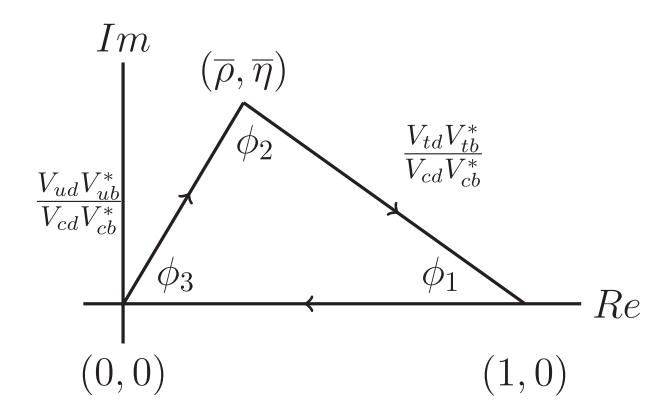
\includegraphics[height=6cm]{UT}
	\caption{The unitary triangles of CKM\cite{ckmfitter}.}
	\label{fig:ckm_angles}
\end{figure}
\begin{eqnarray}
\bar{\rho}+i\bar{\eta}=- \frac{V_{ud}V^*_{ub}}{V_{cd}V^*_{cb}}\label{eq:ckm-rho1}\\
1-(\bar{\rho}+i\bar{\eta})=-\frac{V_{td}V^*_{tb}}{V_{cd}V^*_{cb}}\label{eq:ckm-rho2}
\end{eqnarray}
These angles are obtained by drawing the $(\bar{\rho},\bar{\eta})$ on the complex coordinates, and they are also well-known in the names as: $\phi_1=\beta,\phi_2=\alpha,\phi_3=\gamma$. The results presenting the measurement of CKM angles or $(\bar{\rho},\bar{\eta})$ in 2019 are shown in Figure \ref{fig:ckm19}.
\begin{figure}[htbp]
	\centering
	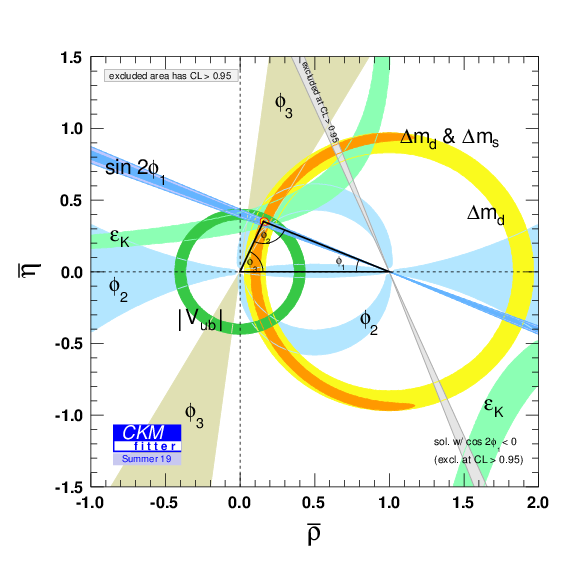
\includegraphics[height=8cm]{ckm19}
	\caption{The CKM triangle fit in the complex plane of $\bar{\rho}-\bar{\eta}$.\cite{ckmfitter}}
	\label{fig:ckm19}
\end{figure}

The measurement of $\phi_1$ and $\phi_2$ are mainly obtained from the time-dependent $CP$ violations (TDCPV) measurement. The $\phi_1$ in the tree-level dominated decays has been precisely measured due to the small hadronic uncertainties. Flavor-Changing-Neutral-Current (FCNC) processes can rise through the $B^0_d-\bar{B^0_d}$ mixing in box diagram, and it's believed that potential NP processes might contribute to the difference in between results of CKM angles measured from experiments, such as $\phi_1$ value in tree-dominated processes and penguin-dominated processes, where both involve $b\to s$ transition. It requires the precise measurements on multiple decay channels to search for the potential NP effects. The prospective large Belle II data and improved detector performance will be much useful to help the discovery of NP in future. 

\section{Time Dependent $CP$ violation}
\subsection{ $CP$ violation in neutral $B$ system}
The  $\phi_1$, $\phi_2$ and $\phi_3$ are essentially measuring the CKM $CP$ violating phase since there's only one complex phase in the CKM matrix and it can be determined by these three angles. 
For determining the value of $\phi_1$, TDCPV measurements provide a good experimental environment.  
From Figure \ref{fig:ckm_angles}, one can obtain $\phi_1$ and $\phi_2$ by Equation \ref{eq:phi1} and \ref{eq:phi2}.
\begin{eqnarray}
\phi_1=Arg(-\frac{V_{td}V^*_{tb}}{V_{cd}V^*_{cb}}) \label{eq:phi1}\\
\phi_2=Arg(-\frac{V_{td}V^*_{tb}}{V_{ud}V^*_{ub}})\label{eq:phi2}
\end{eqnarray}

The time-dependent $CP$ violation comes from the interference of neutral $B$ mixing phase and the weak phase in the decay amplitude. The mass eigenstates which are driving the propagation of neutral $B$ meson states with mixing are: $|B\rangle_{H,L}=p|B\rangle \pm q|\overline{B}\rangle $, where $H$ and $L$ stand for the heavier and lighter mass eigenvalues. The $|B\rangle$ and $|\overline{B}\rangle$ present the flavor eigenstates of neutral $B$ mesons.
The Hamiltonian matrix can be written using flavor eigenstates as shown in Equation \ref{eq:ham_flv}.
\begin{equation}\label{eq:ham_flv}
M_\Gamma=
\begin{bmatrix}
m-i/2\Gamma & M_{12}-i/2\Gamma_{12}\\
M^*_{12}-i/2\Gamma^*_{12}& m-i/2\Gamma 
\end{bmatrix}
\end{equation}
Considering the time evolution of mass eigenstates, the time-dependent states can be shown as Equation \ref{eq:Bht} and \ref{eq:Blt} by using the notation of $B_{H,L}$ as physical states at $t = 0$).
\begin{eqnarray}
B_H(t)=e^{-im_Ht}e^{-\Gamma_Ht/2}B_H \label{eq:Bht}\\
B_L(t)=e^{-im_Lt}e^{-\Gamma_Lt/2}B_L\label{eq:Blt}
\end{eqnarray}
where $M_{H,L}$ and $\Gamma_{H,L}$ are the masses and decay widths of two mass eigenstates. By expanding the mass eigenstates using flavor eigenstates, which are shown in Equation \ref{Bt} and \ref{Bbart}.
\begin{eqnarray}
B(t)=(1/2p)e^{-im_Ht}e^{-\Gamma_Ht/2}(pB+q\bar{B})+(1/2p)e^{-im_Lt}e^{-\Gamma_Lt/2}(pB-q\bar{B}) \label{Bt}\\
\bar{B}(t)=(1/2q)e^{-im_Ht}e^{-\Gamma_Ht/2}(pB+q\bar{B})-(1/2q)e^{-im_Lt}e^{-\Gamma_Lt/2}(pB-q\bar{B})\label{Bbart}
\end{eqnarray}
Replacing $g_{\pm}(t)=\frac{1}{2}(e^{-im_Ht-\Gamma_H/2t}\pm e^{-im_Lt-\Gamma_L/2t})$, Equation \ref{Bt} and \ref{Bbart} become Equation \ref{eq:Bt_new} and \ref{eq:Bbart_new}.
\begin{eqnarray}
B(t)=g_{+}(t)B +\frac{q}{p}g_{-}(t)\bar{B} \label{eq:Bt_new}\\
\bar{B}(t)=g_{+}(t)\bar{B} + \frac{p}{q}g_{-}(t){B}\label{eq:Bbart_new}
\end{eqnarray}
Considering all the phase-spaces of the decay from flavor eigenstates to final states $f(\bar{f})$ are included in the amplitudes $\mathcal{A}_f (\bar{\mathcal{A}}_f)$, one needs to expand the flavor eigenstates using the final states amplitudes to have the differential decay rate $\Gamma(B\to f,t)$. From $B(t) \propto \mathcal{A}_f\psi_f+h.c $ and $ (\bar{B}(t) \propto \bar{\mathcal{A}_f}\psi_{\bar{f}}+h.c)$, combined with Equation \ref{eq:Bt_new} and \ref{eq:Bbart_new}, the decay rate can be shown in Equation \ref{eq:gamma_B} and \ref{eq:gamma_Bbar}.
\begin{eqnarray}
\Gamma(B\to f,t)=|\mathcal{A}_f|(|g_+(t)|^2+|\lambda_f|^2|g_-(t)|^2+2Re(\lambda_f g^*_+(t)g_-(t))) \label{eq:gamma_B}\\
\Gamma(\bar{B}\to \bar{f},t)=|\bar{\mathcal{A}_{\bar{f}}}|(|g_+(t)|^2+|\bar{\lambda}_{\bar{f}}|^2|g_-(t)|^2+2Re(\bar{\lambda}_{\bar{f}} g^*_+(t)g_-(t)))\label{eq:gamma_Bbar}
\end{eqnarray} where the parameter $\lambda_f$ and $\bar{\lambda}_{\bar{f}}$ can be defined as Equation \ref{eq:lambda_f} and \ref{eq:lambda_fbar}.
\begin{eqnarray}
\lambda_f \equiv (q/p) (\bar{\mathcal{A}}_f / \mathcal{A}_f) \label{eq:lambda_f}\\
\bar{\lambda}_{\bar{f}} \equiv (q/p) ( \mathcal{A}_{\bar{f}}/\bar{\mathcal{A}}_{\bar{f})} \label{eq:lambda_fbar}
\end{eqnarray} 
The $q/p$ is introduced by the coefficient of mass eigenstates from weak eigenstates. Using the Hamiltonian matrix, $q/p$ can be presented using Equation \ref{eq:qp}
\begin{equation}\label{eq:qp}
	q/p = \frac{\Delta M - i/2 \Delta \Gamma}{2(M_{12}- i/2 \Gamma_{12})}
\end{equation}
where the $M_{12}$ and $\Gamma_{12}$ stands for the contribution of non-diagnosed term in the Hamiltonian matirx. $\Delta{M}=M_H-M_L$ and $\Delta{\Gamma}=\Gamma_H-\Gamma_L$ are the difference of mass and decay width for two mass eigenstates, respectively.
It's obvious that if $|A_f| \neq |\bar{A}_{\bar{f}}|$, direct $\it{CP}$ violation will occur.  
The time-dependent decay rate difference is defined as Equation \ref{Acp}.
\begin{equation}\label{Acp}
\begin{split}
A_{CP}(t)&\equiv \frac{\Gamma(B\to f,t)-\Gamma(\bar{B}\to \bar{f},t)}{\Gamma(B\to f,t)+\Gamma(\bar{B}\to \bar{f},t)}\\
&=\frac{\mathcal{S} sin(\Delta{M}t)-\mathcal{A}cos(\Delta{M}t)}
{cosh(\Delta \Gamma t/2)+A^f_{\Delta \Gamma}sinh(\Delta \Gamma t/2)}
\end{split}
\end{equation}
where
\begin{eqnarray}\label{cp-parameters}
\mathcal{S}=\frac{2Im(\lambda_f)}{1+|\lambda_f|^2} \label{eq:S}\\
\mathcal{A}=\frac{1-|\lambda_f|^2}{1+|\lambda_f|^2}\label{eq:A}\\
A^f_{\Delta \Gamma}=-\frac{2Re(\lambda_f)}{1+|\lambda_f|^2}
\end{eqnarray}
From Equation \ref{eq:S} and \ref{eq:A}, the time-dependent CP violation parameters $\mathcal{S}$ and $\mathcal{A}$ are dependent on the parameter $\lambda_f$.

\subsection{$\phi_1$  from $B^0 \to J/\psi K^0_S$}
If final states are $CP$ eigenstates, the amplitudes are obtained by $\mathcal{A}_f \equiv \langle f|H|B\rangle$ and $\bar{\mathcal{A}_f} \equiv \langle f|H|\bar{B}\rangle$. In $B_d^0-\bar{B_d^0}$ mixing system, the $q/p$ can be treated as $e^{i\phi_d}$ as a pure phase term. This relative phase accounts the transition from $b$ to up-type quarks to strange quark $s$ in mixing, so it can be presented as $\phi_d = \text{Arg}(V^*_{td}V_{tb})/(V^*_{tb}V_{td}) \approx 2\phi_1 $ based on negligible correction to the SM. In mode $B^0 \to J/\psi K^0_S$, considering $\Delta \Gamma$ can be treated as zero in the SM in this case\cite{dighe2001width}, Equation \ref{Acp} can be reduced to Equation \ref{eq:acp}.

\begin{equation}\label{eq:acp}
	A_{CP}(t)=\mathcal{S} \text{sin}(\Delta{M}t)- \mathcal{A}\text{cos}(\Delta{M}t)
\end{equation}

\begin{comment}
Usually, $S_f$ provides a good sensitivity to $\phi_1$ in Eq(1.42) by replacing $\phi_d$ inside $\lambda_f$ since the rest two equations canceled out the complex phase of $(q/p)$. For instance, in the process of  $b\to \bar{c}cs$ ,the amplitude contributions from tree level and loop level diagram can be written in a form as follows using the CKM unitary condition: 
\end{comment}
which receives contributions from tree-level and loop-level processes shown in Figure \ref{fig:jpsiks} , 

\begin{figure}[htpb]
	\centering
	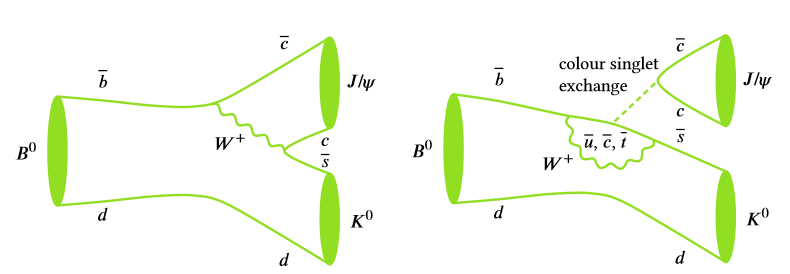
\includegraphics[height=4cm]{jpsiks-diagram}
	\caption{The dominated tree-level (left) and the suppressed loop-level (right) of $B\to J/\psi K^0$, in which $K^0$ particles are detected $K_S^0$\cite{wishahi2014measurement}.}
	\label{fig:jpsiks}
\end{figure}

%\begin{equation}
%	\mathcal{A}_f= 
%	\lambda^s_c T_f + 
%	\lambda^s_u P_f; \\
%	\lambda^q_i = V^*_{ib}V_{iq}
%\end{equation}
%where $T_f$ and $P_f$ stands for leading order contribution of tree and penguin diagrams, see Fig(1-7). Here, the leading term can be presented as: 

Using the relation $|V_{ub}|\ll |V_{cb}|\ll|V_{us}|<|V_{cs}|$, it's obvious that $V^*_{ub}V_{us} \ll V^*_{cb}V_{cs}$, so the penguin-mode is suppressed in the Standard Model. The $\eta_f$ is defined as the $\it{CP}$ eigenvalue. Given $\eta_f=1$ and $|\lambda_f|=1$ in $B^0 \to J/\psi K^0_S$, from \ref{cp-parameters}, $\it{CP}$ violation parameters can be presented as shown in Equation \ref{SA}.
\begin{equation}\label{SA}
\mathcal{S} = Im(\lambda_f)
=-sin(\phi_d)\eta_f=sin(2\phi_1) ; \: \mathcal{A} = 0
\end{equation}

From Equation \ref{SA} , $\phi_1$ can be obtained precisely in the measurement of time-dependent $\it{CP}$ violation in $B^0 \to J/\psi K^0_S$.
\begin{comment}
In the $b\to q\bar{q}s$ process where flavor $q$ is not charm, similar to the discussion above, we can extract $\phi_1$ using the same method. Moreover, it provides a penguin-dominated process which is sensitive to the contribution of New Physics, which includes the $B^0_d\to K^0_S K^0_S K^0_S$ decay. In the next section, it's clear that such decay process is important to provide additional insight in seeking the effect beyond the SM (BSM contribution).
\end{comment}



\subsection{$\phi_1$ from penguin-dominated mode $b\to q\bar{q}s$}
Compared to $B^0 \to J/\psi K^0_S$ channel, the measurement of $\mathcal{S}$ and $\mathcal{A}$ from penguin-dominated channels through $b \to q\bar{q}s$ where $q$ is $u,d,s$ can be different due to the varied tree-to-penguin amplitude ratio. Furthermore, they are quite sensitive to NP effects for the following reasons\cite{b2book}. First, they can probe $B^0-\bar{B}^0$ mixing through different short-distance vertices compared to the tree-level dominated decays. Second, the tree-level decay amplitude is suppressed and penguin-level amplitude is dominated, while the overall non-NP amplitude is relatively small so NP effects may show up easier. Last but not least, they comprise a large number of different final states, which can help disentangling non-perturbation long-distance physics from short-distance information, such as $\phi_1$ or NP contributions to the weak Hamiltonian. 

\begin{comment}
First,  the $b\to q\bar{q}s$  gives a different vertex in gluonic decay than tree diagram. 
Second, such process is tree level suppressed but penguin-dominated, so the New Physics effects can be easier to be spotted. The SM agrees with tree level process in percent accuracy so the sub-percent BSM effects may be hard to see. Similar to Fig(1-7), due to FCNC tree level forbidden, 
\begin{figure}[H]
\centering
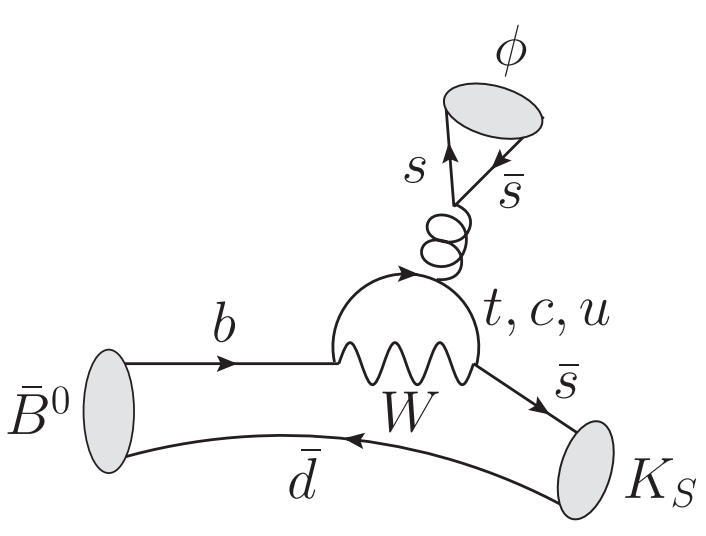
\includegraphics[height=5cm]{Bto3Ks}
\caption{penguin mode $b\to q\bar{q}s$ where $\phi$ is formed by two strange quark as the intermediate state.}
\end{figure}

\end{comment}
Considering possible New Physics contribution besides the tree-level and penguin-level processes as $A_f^{NP}$, the decay amplitude can be rendered as Equation \ref{eq:Af_NP} 
\begin{equation}\label{eq:Af_NP}
\mathcal{A}_f= 
\lambda^s_u T_f + 
\lambda^s_c P_f +
{A}_f^{NP} 
\end{equation}
where $T_f$ and $P_f$ are tree-level and penguin-level amplitudes. The coefficients $\lambda^s_u$ and $\lambda^s_c$  are determined from CKM matrix elements by $\lambda^q_i \equiv V^*_{ib}V_{iq}$. Note that compared to the $B^0 \to J/\psi K^0_S$,
the tree level amplitude $T_f$ is suppressed and penguin amplitude $P_f$ is dominated in $b\to q\bar{q}s$. It is also worth noting that $T_f$ contains tree-level $W^{\pm}$ exchange, QCD and electroweak penguin contributions. These carry the combination of CKM matrix elements $\lambda_t^s = V_{ts}V^*_{tb}=-(1+\epsilon_{uc})\lambda^s_c$ where $\epsilon_{uc} \equiv \lambda^s_u / \lambda^s_c = \mathcal{O}(\lambda^2)$. In the SM with neglected $\epsilon$,  $b\to q\bar{q}s$ modes are pure penguin with the same weak phase as $B^0 \to J/\psi K^0_S$ has. Thus, direct $CP$ violation vanishes and time-dependent $CP$ violation reflects $\mathcal{S}$ in the same way as $B^0 \to J/\psi K^0_S$ does. 

Departures from this limit, non-neglected tree amplitude $T_f$ (often called ``tree pollution"), as well as possible NP effects, could give different results on $\phi_1$. The $\phi_1$ differences can be reflected by the $\mathcal{S}$ difference, hence $\Delta S$ is defined as Equation \ref{eq:ds}.

\begin{equation}\label{eq:ds}
\Delta S = \mathcal{S}_{f} - \mathcal{S}_{J/\psi K^0_s}
\end{equation}

Introducing the tree-penguin ratio $r^T_f = T_f / P_f$, NP-to-SM ratio $r^{NP}_f = \mathcal{A}^{NP}_f / (\lambda^s_c P_f)$, the following statements are usually used\cite{b2book}:

\textbullet \space Branching ratios are affected at $\mathcal{O}(|\epsilon_{uc}r^T_f|,|r^{NP}_f|)$

\textbullet \space Direct CP violation in the SM are of $\mathcal{O}(\epsilon_{uc}\text{Im}(r^T_f))$


\textbullet \space $-n^{CP}_f\mathcal{S} = \text{sin}(2\phi_1) + \Delta \mathcal{S}$, where
$\Delta \mathcal{S}=2{cos}2\phi_1 {sin}\phi_3 |\epsilon_{uc}| \text{Re}(r^t_f) + \Delta \mathcal{S}^{NP}$.
This suggests that non-zero $\Delta S$ without the NP effect is still allowed in a small scale within the SM.
Therefore, in the precised measurement using the future Belle II data, it's important to understand $\Delta S$ within the SM correction to properly explain the experiment results. The $\Delta S$ should be larger than the SM allowed value by $5\sigma$ to be called as the evidence of the NP, where $\sigma$ is the total uncertainty of $\Delta S$.

\subsection{$\phi_1$ from $B^0 \to K_S^0  K_S^0  K_S^0$}% 2021.01.25 ends
Since the Belle experiment reported the time-dependent $\it{CP}$ analysis on various $b\to q\bar{q}s$ which experimentally showed that the difference on $\phi_1$ has a margin for NP effects\cite{chen2007observation}, the improved measurements with a larger data collection is popularly discussed in order to reduce the impact of uncertainties and clear the tension between results. The decay channel $B^0 \to K_S^0  K_S^0  K_S^0$ is one of the most promising modes for this purpose. The $\it{CP}$ eigenvalue of $B^0 \to K_S^0  K_S^0  K_S^0$ is positive ($CP$ eigenvale $=+1$).  There's no up-quark shown in the final states, the potential contribution of $b\to u\bar{u}s$ re-scattered into $b\to s\bar{s}s$ is almost of absence, which makes $B^0 \to K_S^0  K_S^0  K_S^0$ a much cleaner channel compared to $B^0 \to K^+  K^-  K_S^0$\cite{gershon2004time}. In all final states with three $K_S^0$ from a neutral $B$ decay, the phase-space based decay process and the resonant decay process such as $B^0\to f_0(980)K_S^0(f_0(980)\to K_S^0 K_S^0)$ are shown in the left and middle of Figure \ref{fig:3ksfey}, which all yield $\it{CP}$-even states treated as signal events. In the meanwhile, $b\to c \to s$ can also produce the final states with three $K_S^0$ through a tree-level process like $B^0\to \chi_{c0}K_S^0(\chi_{c0}\to K_S^0 K_S^0)$ with a different weak phase and $\it{CP}$-odd states, as shown in the right of Figure \ref{fig:3ksfey}. Such a tree-level process is treated as background and can be rejected by applying veto on two $K_S^0$ invariant mass within $\chi_{c0}$ mass window, which is considered as a minor background at the current luminosity. Due to the same weak phase in the decay amplitudes, any potential NP effects expected in the $B^0 \to \phi K^0_S$ and $B^0 \to \eta^{'} K^0_S$ should also affect $B^0 \to K_S^0  K_S^0  K_S^0$ and the absence of NP effects will lead the close $\it{CP}$ violation as $J/\psi K^0_S$\cite{gershon2004time}. To be noted, as discussed in the previous section that the SM correction due to the different tree-penguin ratio, $B^0 \to \eta^{'} K^0_S$, $B^0 \to \phi K^0_S$ and  $B^0 \to K_S^0  K_S^0  K_S^0$ modes could create non-zero $\Delta \mathcal{S}$ in a slightly different level.
There were attempted theoretical calculation based on the QCD model for the $\Delta \mathcal{S}$ in these modes. 
For $B^0 \to \eta^{'} K^0_S$ and $B^0 \to \phi K^0_S$, the details about such a calculation on $\Delta \mathcal{S}$ within the SM can be find in Ref.$\sim$\cite{Beneke_2003}. As for $B^0 \to K_S^0  K_S^0  K_S^0$, the calculation of $\Delta \mathcal{S}$ within the SM can be find in Ref.$\sim$\cite{PhysRevD.72.094003}. In general, the expected SM-allowed $\Delta \mathcal{S}$ from QCD model suggests the upper limit at $\sim 0.05$ for $B^0 \to \phi K^0_S$, $0.03$ for $B^0 \to \eta^{'} K^0_S$, and $0.06$ for $B^0 \to K_S^0  K_S^0  K_S^0$. For $B^0 \to K_S^0  K_S^0  K_S^0$, the theoretical uncertainty is expected to be small compared with the experimental uncertainties. Thus, in the comparison of SM-allowed $\Delta S$ and the experimental results, we current only focus on the statistical and systematic uncertainties from the experiment and ignore the  QCD model uncertainty.  The theoretical calculation suggests the positive sign of $\Delta \mathcal{S}_{3K^0_S}$. We take $\Delta \mathcal{S} \sim 0.05$ as the SM-allowed upper limit predicted by the QCD model. 


 \begin{figure}[htpb]
 	\centering
	\begin{minipage}[t]{0.32\linewidth}
		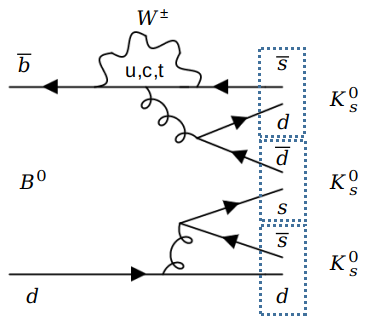
\includegraphics[width=1\linewidth]{fey1}
	\end{minipage}
	\begin{minipage}[t]{0.32\linewidth}
		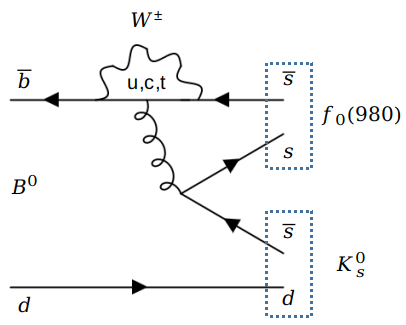
\includegraphics[width=1\linewidth]{fey2}
	\end{minipage}
\begin{minipage}[t]{0.32\linewidth}
	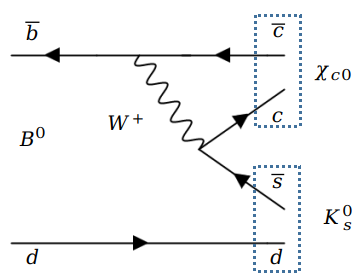
\includegraphics[width=1\linewidth]{fey3}
\end{minipage}
	\caption{}
	\label{fig:3ksfey}
\end{figure}

The current result of  $B^0 \to J/\psi K_S^0$ using the full Belle data is presented as $\mathcal{S}_{J/\psi K^0_S} = + 0.670 \pm 0.029 (\text{stat}) \pm 0.013(\text{syst})$\cite{b2book}. In the meantime, the latest result from $B^0 \to K_S^0  K_S^0  K_S^0$ using the full Belle data\cite{kang2020measurement} is presented as: $\mathcal{S}_{3K^0_S} = - 0.71 \pm 0.23 (\text{stat}) \pm 0.05(\text{syst})$, and the result from BaBar \cite{Lees:2011nf} is: $\mathcal{S}_{ 3K^0_S} = - 0.94 ^{+0.21}_{-0.24} (\text{stat}) \pm 0.06(\text{syst})$. Both results have shown a small deviation from the result in $B^0 \to J/\psi K_S^0$ while the statistical uncertainties are much dominated which prevents the claim about whether NP effects are existed. For $\Delta \mathcal{S}$ from $B^0 \to K_S^0  K_S^0  K_S^0$, the experimental sensitivity of $\Delta \mathcal{S}$ will be dominated by $\mathcal{S}_{3K^0_S}$ uncertainty because the total uncertainty from $J/\psi K^0_S$ will be reduced to  $\sim0.005$ at $50 \: \text{ab}^{-1}$ Belle II data\cite{b2book}, which is negligible. The Figure \ref{fig:sensitivity} shows the expected $\Delta \mathcal{S}$ uncertainty from the Belle II technical design report with respect to the luminosity in future Belle II\cite{Abe:2010gxa}, which requires that the Belle II results should be prepared for $\Delta \mathcal{S} < 0.2$ caused by the NP effects. The curves are extrapolated based on the Belle results from 492 fb$^{-1}$ data and take into account the reducible systematic and statistical uncertainties\cite{aushev2010physics}. The Table \ref{tab:sensitivity} shows the corresponding total uncertainties of $\Delta \mathcal{S}$ in Figure \ref{fig:sensitivity} at 0.5 ab$^{-1}$, 5 ab$^{-1}$ and 50 ab$^{-1}$ luminosity. For $B^0 \to K_S^0  K_S^0  K_S^0$ at 50 ab$^{-1}$ , if $\Delta \mathcal{S}_{3K^0_S} \sim 0.25$, the total uncertainty should be less than $0.04$ to claim a $5\sigma$ deviation from the SM upper limit 0.05 for the appearance of the NP effects, which is close to the expected total uncertainty in Table \ref{tab:sensitivity}.

\begin{figure}[H]
	\centering
	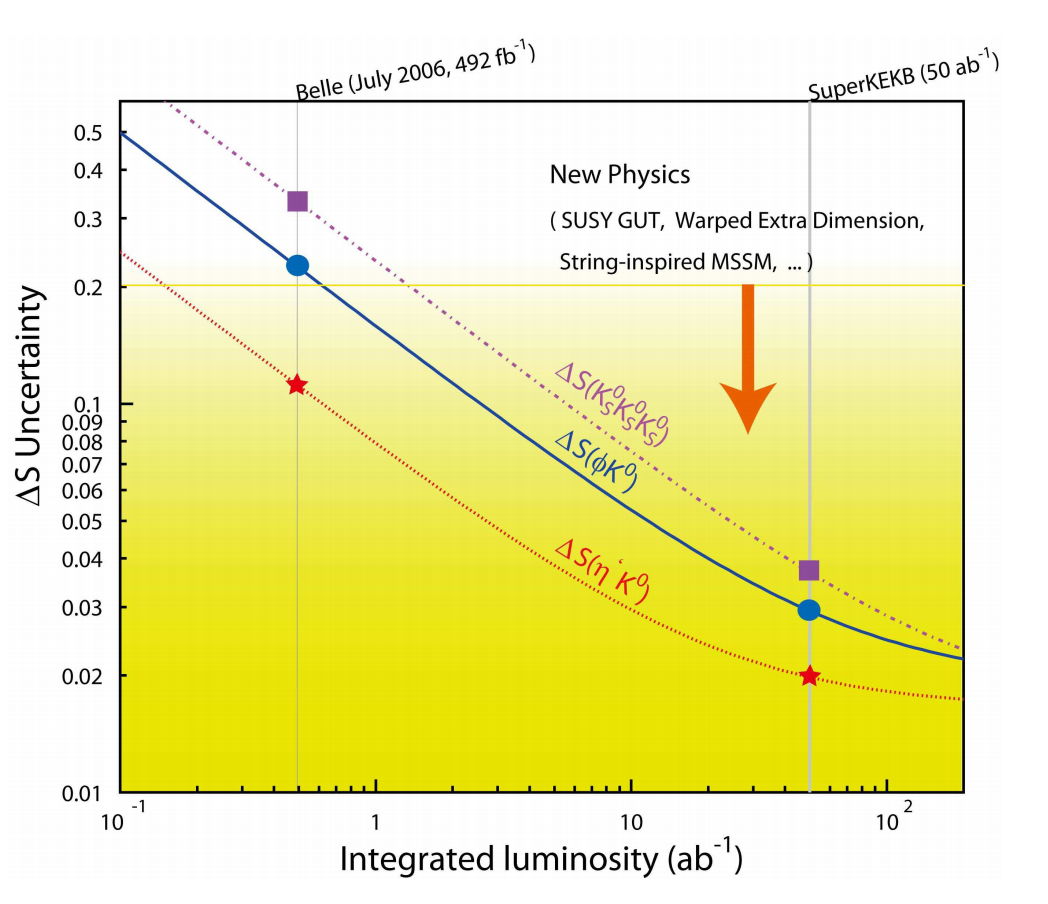
\includegraphics[height=10cm]{sensitivity}
	\caption{Expected  sensitivity of $\Delta \mathcal{S}$ with respect to the integrated luminosity of the Belle II future data from the Belle II technical design report\cite{Abe:2010gxa}.}
	\label{fig:sensitivity}
\end{figure}

\begin{table}[H]
	\centering
	\large
	\caption{$\Delta \mathcal{S}$ estimated total uncertainties with respect to the integral luminosities in the Belle II technical design report\cite{Abe:2010gxa}. Three decay modes receive the same potential NP effects due to the same weak phases involved in the decay processes\cite{gershon2004time}.}
	\label{tab:sensitivity}
	\begin{tabular}{c c c c}
		\toprule
		Observable & Belle ($0.5 \: \text{ab}^{-1}$) & Belle II ($5 \: \text{ab}^{-1}$)& Belle II ($50 \: \text{ab}^{-1}$)\\
		\hline
		$\Delta \mathcal{S}_{\phi K^0_S}$ & 0.22 &  0.073 & 0.029\\
		$\Delta \mathcal{S}_{\eta' K^0_S}$   & 0.11 &  0.038 & 0.020\\
		$\Delta \mathcal{S}_{ K^0_S K^0_S K^0_S}$ & 0.33 & 0.105 & 0.037\\
		\bottomrule
	\end{tabular}
\end{table}

\begin{comment}
As the main decay process that have been studied in this thesis, $B^0_d\to K^0_S K^0_S K^0_S$ propagates through $b\to \bar{s}ss$ as well. There are more than one process that will yield the same final states ($3K_S^0$). The difference here is that $3K_S^0$ final states can be produced not only from the $ss$ intermediate state like $f_0(980)$ through penguin mode, but also viable from charm decay (see Fig(1-10)), which $\bar{c}c$ comes from tree level transition. The contribution from tree level process is estimated to be small but must be aware of using Dalitz analysis in future. Similarly, the $\bar{s}s$ intermediate decay, such as $B^0 \to f_0(980)K^0_S$, would also give the same $\it{CP}$-eigenvalue in final states, which is also considered as signal because of $\it{CP}$-even), while $b\to c\to s$ tree level is considered as background that yields $\it{CP}$-odd final states. The previous result in this channel from Belle full dataset \cite{kang2020measurement} is:  $\mathcal{S}$ = -sin2$\phi_1$ = $-0.72\pm 0.23(stats)\pm 0.05(syst)$ and $\mathcal{A}=0.12\pm0.16(stats)\pm 0.05(syst)$. The earlier results from Babar\cite{lees2012amplitude} is: $\mathcal{S}$ = -sin2$\phi_1$ = $-0.94^{+0.21}_{-0.24}(stats)\pm 0.06(syst)$. The results are mostly limited by the statistical uncertainty with minor difference. With the expected luminosity from Belle II in future, we are able to cut off the margin in between the results and the Standard Model. This thesis, as the first trial to perform the $\it{CP}$ measurement on this channel for Belle II, is inevitably dominated by the low data size in the early operation, but will show the good capability and potential in the analysis tools and methods towards the promising future.
\end{comment}

% 2021.01.26 ends move below to the chapter 3

\begin{comment}
\begin{figure}[h]
\begin{minipage}[t]{0.33\linewidth} % 如果一行放2个图,用0.5,如果3个图,用0.33
\centering 
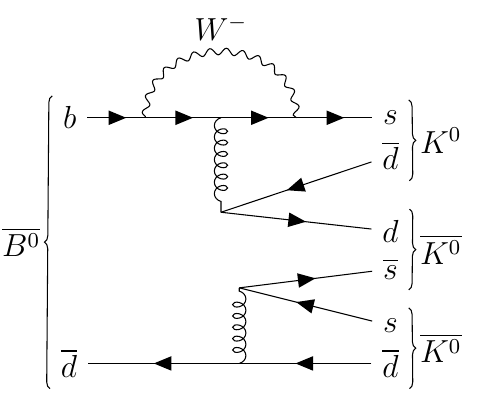
\includegraphics[height=4cm]{feynman3Ks01} 
\label{fig:side:a} 
\end{minipage}%
\begin{minipage}[t]{0.33\linewidth} 
\centering 
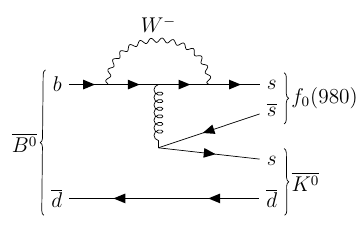
\includegraphics[height=4cm]{feynman3Ks02} 
%\caption{ } 
\label{fig:side:b} 
\end{minipage}% 
\begin{minipage}[t]{0.33\linewidth} 
\centering 
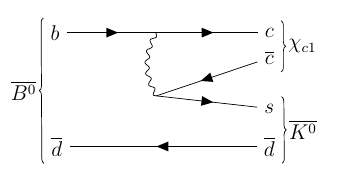
\includegraphics[height=3cm]{feynman3Ks03} 
%\caption{ } 
\label{fig:side:a} 
\end{minipage} %
\caption{non-resonant signal (left),resonant signal (middle) and tree-level resonant backgrounds (right)
$B^0_d\to3K^0_S$ diagrams}.
\end{figure}
\end{comment}



\begin{comment}
\begin{tikzpicture}
\begin{feynman}
\vertex (a1) {\( b\)};
%\vertex[right=1cm of a1] (a2);
\vertex[right=2cm of a1] (a3);
%\vertex[right=1cm of a3] (a4) ;
\vertex[right=2cm of a3] (a5) {\(c\)};
\vertex[below=1.25cm of a3] (a6) ;
\vertex[below=0.5cm of a5] (a7) {\(\overline{c}\)};
\vertex[below=1.5cm of a5] (a8) {\(s\)};
\vertex [below=0.75cm of a8] (b1) {\(\overline{d}\)};
%\vertex [left=2cm of b1] (b2);
\vertex [left=4.2cm of b1] (b3) {\(\overline{d}\)};
%\vertex [above=1cm of b2] (b4);
%\vertex [above=0.5cm of b1] (b5) {\({s}\)};
%\vertex [above=1.25cm of b1] (b6) {\(\overline{s}\)};
\diagram*{
{[edge=fermion],
(a1)--(a3)--(a5),
(b1)--(b3),
(a7)--(a6)--(a8),
%(b5)--(b4)--(b6),
},
%(b2)--[gluon] (b4),
(a3)--[photon, bend right] (a6),
%(a2)--[boson, half left,edge label=\(W^{-}\)] (a4)
};
\draw [decoration={brace}, decorate] (b3.south west) -- (a1.north west)
node [pos=0.5, left] {\(\overline{B^{0}}\)};
\draw [decoration={brace}, decorate]  (a8.north east)--(b1.south east) node [pos=0.5, right] {\(\overline{K^{0}}\)};
\draw [decoration={brace}, decorate]  (a5.north east)--(a7.south east) 
node [pos=0.5, right] {\(\chi_{c1}\)};
%\draw [decoration={brace}, decorate]  (a8.north east)--(b6.south east) 
%node [pos=0.5, right] {\(\overline{K^{0}}\)};
\end{feynman}
\end{tikzpicture}
\end{comment}
